%%%%%%%%%%%%%%%%%%%%%%%%%%%%%%%%%%%%%%%%%%%%%%%%%%%%%%%%%%%%%%%%%%%%%%%%%%%%%%%%
Fruit detection is a fundamental and crucial task for automating yield mapping. As it is a precursor to many other tasks (e.g counting, tracking, etc.), its accuracy is critical to the performance of the overall system. In the detection stage, the goal is to identify pixels that are likely to belong to fruit. Specifically, the detection algorithm takes as input an RGB image and produces a binary mask where pixels belonging to fruit are marked as ones and all other pixels are marked as zeros.

Varying colors at different stages, different lighting conditions, shadows and occlusions created by leaves and branches make the job of identifying fruit from images difficult. Earlier methods for fruit detection relied on color thresholds and controlled lighting. More recent techniques are being dominated by deep-learning-based approaches ~(\cite{chen_counting_2017, hani_apple_2018}). The overwhelming success of these techniques is often attributed to the huge amount of training data from which the networks learn features that ideally generalize across environments. Obtaining such data in cluttered environments such as orchard settings though is tedious and cumbersome. Labeling a $1920\times1080$ image can take up to $15$ minutes depending on the number of apples in it. Therefore, it is important to quantify the improvement in detection and counting performance by deep network-based models compared to simpler, classical methods.


In this chapter, we present two different methods for fruit detection. First, we present a semi-supervised color-based clustering technique using Gaussian Mixture Models (GMM) and Expectation-Maximization (EM)~\cite{em}. This method utilizes minimal user interaction to train a classification model and uses it to identify the fruits. The system can store trained models that can be used for a similar variety of fruit and lighting conditions. It also utilizes multiple views for detection based on the assumption that for every apple there is some view from which it is detected. This provides robustness against false positives and leads to high precision and recall.

Second, we present a novel approach based on a pixel-wise segmentation network, U-Net~\cite{ronneberger_u-net:_2015}. We provide details for implementation and rationale for design choices. We perform a thorough side-by-side evaluation of these methods. Additionally, we compare their performance to the work of Bargoti et al.~\cite{bargoti_deep_2017} which is based on a state-of-the-art object detection network- Faster R-CNN (FRCNN)~\cite{ren_faster_2015}.



%%%%%%%%%%%%%%%%%%%%%%%%%%%%%%%%%%%%%%%%%%%%%%%%%%%%%%%%%%%%%%%%%%%%%%%%%%%%%%%%
\begin{figure}[!hbpt]
\includegraphics[width = .18\columnwidth]{figures/detection/dataset11.jpg}          
\includegraphics[width = .18\columnwidth]{figures/detection/dataset222.jpg}           
\includegraphics[width = .18\columnwidth]{figures/detection/green_apples_typical11.png}           
\includegraphics[width = .18\columnwidth]{figures/detection/dataset20151.jpg}           
\includegraphics[width = .18\columnwidth]{figures/detection/shady11.png}           
   \caption[Typical conditions in orchard settings.]{Conditions typical to orchard settings. Our semi-supervised detection algorithm performs well in the first four cases. For the final image, it requires a significant amount of user supervision to obtain reasonable performance.}
   \label{fig:Conditions}
\end{figure} 
\section{A Semi-supervised Approach for Fruit Detection}\label{sec:segmentation}

One approach to detection is to simply choose fruit pixels based on predetermined thresholds on color values. While this approach has the advantage of simplicity, in field conditions it often fails due to the variability of lighting conditions. In recent years,  Fully Convolutional Networks (FCN) trained for pixel-wise prediction has gained popularity for fruit and crop segmentation (\cite{chen2017counting}). While these models achieve high accuracy, training a network general enough to accommodate variations in light and visibility conditions remains challenging. Further, training FCN’s for each orchard video separately requires a significant amount of human labor involved in generating ground truth labels for each apple.

We propose a semi-supervised detection method based on color and shape features of fruit. By itself, the detection algorithm runs at $5$ to $6$ frames per second on images of size $1920 \times 1080$ and $15$ frames per second for images of the size of $640 \times 480$ on a DELL XPS laptop with $16$GB RAM and $2$GB GPU memory. The training required by the user is minimal. It is assisted by a simple, convenient user interface. The method generalizes well for the cases where the training and testing data are from different portions of an orchard taken on different days. This method is expected to work for cases where fruit is visibly distinguishable from the surrounding vegetation based on the color. Some working and challenging conditions are shown in Fig.~\ref{fig:Conditions}. 

\begin{figure}[!hbpt]
\centering
    \includegraphics[width= \columnwidth]{figures/detection/all_semantic_entities1.pdf}                  
    \caption[Gaussian representation of semantic entities.]{Gaussian representation of semantic entities. Each blue data point is the mean LAB color for each superpixel in the image. Each $3D$ ellipsoid represents the Gaussian fit on clusters obtained from unsupervised clustering using EM and GMM. For visualization, showing $19\%$ of the standard deviation for each Gaussian ellipsoid. Red-colored ellipsoids are capturing the super-pixels belonging to apples.}
    \label{fig:all_semantic_entities}
\end{figure}

\begin{figure}[!hbpt]
\centering
        \begin{subfigure}{0.45\textwidth}
            \includegraphics[width=\textwidth]{figures/detection/init_and_usage.pdf}           
            \caption{Input is a video. For each frame in the initialization step, among all Gaussian components $G_i$, $G_k$ are chosen and saved in a list using a UI. These saved $G_k$ are used for finding Gaussian components in the usage step.}
             \label{fig:init_and_usage}
         \end{subfigure}\hspace{2cm} \begin{subfigure}{0.4\textwidth}
            \includegraphics[width=\textwidth]{figures/detection/General_paradigm.pdf}                  
        \hspace*{-1cm}\caption{A general way of using the Usage and Initialization phase for a dataset.}       
        \label{fig:General_paradigm}        
        \end{subfigure}
   \caption[User interface for fruit detection based on semi-supervised clustering.]{Explanation of the user interface for fruit detection based on semi-supervised clustering.}
   \label{fig:init_genparadigm}
\end{figure}




\textbf{Details of the segmentation process:} For each frame in the image sequence, we convert it from RGB to LAB (\cite{gauch1992comparison}) color space and perform SLIC superpixel segmentation (Fig.~\ref{fig:seg_pipeline}(\subref{fig:pipe2})) (\cite{achanta2012slic}). This generates a set of superpixels $\mathcal{S}$ for each image.

$$\mathcal{S}=\{\mathbf{s_1},...,\mathbf{s_N}\}$$ 

Here each superpixel $\mathbf{s_i}$ is represented by $\{ \mu^L_i, \mu^A_i, \mu^B_i \}$, the mean L,A,B values for all pixels $\mathbf{s_i}$. We assume that the set $\mathcal{S}$ of superpixels can be modeled as a density function $p(\mathbf{s}|\theta)$ governed by the set of parameters $\theta$. For soft segmentation, we model $\mathcal{S}$ as a Gaussian Mixture Model(GMM)  (\cite{chuang2001bayesian, ruzon2000alpha}) with $M$ components. Hence $p$ is represented by a set of Gaussian components $G_i$ and parameters $\theta$ as the respective mean $\mu_i$ and covariances $\Sigma_i$ for each $G_i$. 

$$ p(\mathbf{s}|\theta)=\sum_{i=1}^M{\alpha_i G_i(\mathbf{s}|\mu_i, \Sigma_i)} $$ such that $\sum_{i=1}^M{\alpha_i}=1$

The likelihood function of the parameters can be written as:

$$ \mathcal{L}(\mu,\Sigma|\mathcal{S}) = \prod_{i=1}^N{p(\mathbf{s_i}|\mu_i,\Sigma_i)} $$

The resultant Gaussian mixture density estimation problem is:

$$(\mu^*, \Sigma^*) = \arg\!\max_{\mu, \Sigma} {\mathcal{L}(\mu,\Sigma|\mathcal{S})} $$

where $\mu^*={\mu^*_1,...,\mu^*_M}$ and $\Sigma^*={\Sigma^*_1,...,\Sigma^*_M}$. Expectation Maximization (EM) is used (\cite{em}) to estimate $\mu^*_i, \Sigma^*_i$ for each Gaussian cluster $G_i$. Each Gaussian cluster $G_i$ thus generated contains similar colored superpixels (Fig.~\ref{fig:all_semantic_entities}) and represents different semantic entities of an orchard frame such as the sky, soil, apples, leaves, branches, etc. 

Next, we identify which among these $G_i$ capture superpixels belonging to apples. We divide this step into two parts: (1)~$\textit{initialization}$ and (2)~$\textit{usage}$ (Fig.~\ref{fig:init_genparadigm}(\subref{fig:init_and_usage})). In the $\textit{initialization}$ phase, we provide an interface for a user to interact with the $G_i$. Here the user is allowed to:
\begin{itemize}
\item select components $G_k$ which completely capture apples. For each selected $G_k$, their respective $\mu_k^*$ and $\Sigma_k^*$ are pushed in a list in memory.
\item delete components from the list stored in memory. This step is generally needed where there is a sudden illumination change and the previous stored components $G_k$ become bad (Fig.~\ref{fig:init_genparadigm}(\subref{fig:General_paradigm})). We can update the old list, and continue the segmentation process from the current frame.
\end{itemize}

In the $\textit{usage}$ phase, the user interface is not invoked. To find components belonging to fruit, we perform a simple matching between the current frame's $G_i$ and the saved $G_k$. We use KL Divergence as the distance measure for comparing Gaussians from $G_i$ and $G_k$. For a matched Gaussian $G_i$, all the superpixels within the $90\%$ confidence bounds are identified as superpixels belonging to fruit. A normal usage paradigm is shown in Fig.~\ref{fig:init_genparadigm}(\subref{fig:General_paradigm}).


\begin{figure*}[!hbpt]
        \centering
        \begin{subfigure}[b]{.23 \textwidth}
            \includegraphics[width=\textwidth]{figures/detection/pipeline1.jpg}           
            \caption{Input image.}
             \label{fig:pipe1}
         \end{subfigure}\hspace{.2cm}\begin{subfigure}[b]{.23 \textwidth}
         %\raggedleft
            \includegraphics[width=\textwidth]{figures/detection/pipeline2.jpg}                  
        \caption{Superpixels.}       
        \label{fig:pipe2}        
        \end{subfigure}\hspace{.2cm}\begin{subfigure}[b]{.23 \textwidth}      
        
         %\raggedleft
            \includegraphics[width=\textwidth]{figures/detection/pipeline5.jpg}                  
        \caption{Segmentation.}       
        \label{fig:pipe4}        
        \end{subfigure}\hspace{.2cm} \begin{subfigure}[b]{.23 \textwidth}
         %\raggedleft
            \includegraphics[width=\textwidth]{figures/detection/pipeline4.jpg}                  
        \caption{Detection.}       
        \label{fig:pipe5}        
        \end{subfigure}
   \caption{Segmentation pipeline.}
   \label{fig:seg_pipeline}
\end{figure*}

The main advantage of this method is the simplicity of annotation. Typically, $10-20$ clicks (user-supervision) are enough to create a classification model to detect all the fruit in a video. However, this method does not work if the fruit is not distinguishable by color from the background. The training model for the GMM can be obtained in a user-supervised or semi-supervised fashion. For the user-supervised model, the first $5$ frames of a given dataset are used to obtain the classification model. For the semi-supervised version, on the other hand, the classification model is obtained from a dataset different from the test sets.


\subsection{A Supervised Approach for Fruit Detection}\label{subsec:unetdetection}
While the semi-supervised color-based clustering technique is intuitive and simple to train, it is hard to generalize across different datasets and it is not useful when fruit are indistinguishable by color. In this section, we present an approach for detecting fruits using pixel-wise semantic segmentation. Each pixel in the image is assigned a class (fruit/background), and our goal is to minimize the total classification error. Currently, there are many solutions for dense semantic segmentation ~\cite{long_fully_2015,badrinarayanan2017segnet}. However, to be effective for fruit detection a solution must have specific capabilities:

\begin{itemize}
    \item As data annotation for fruit trees is difficult, the chosen network architecture must be able to leverage small amounts of training data and utilize the available data efficiently.
    
    \item The design must be able to deal with small objects and occlusions. Fruit is tiny and from a typical imaging distance of $2-3$ meters, often occupy $5 - 50$ pixels in a $1920 \times 1080$ image.
    
    \item The solution must be able to handle class imbalance (the ratio of fruit to background pixels is around $5\% - 15\%$
\end{itemize}

A Convolutional Neural Network (CNN) that achieves high precision and recall for small objects with a small amount of data is U-Net~\cite{ronneberger_u-net:_2015}. U-Net contains a contracting and expanding path, where the contracting path is a typical convolutional network. During the contraction, the spatial information is reduced while feature information is increased. The expansive pathway combines the feature and spatial information through a sequence of up-convolutions and concatenations (skip-connection layers) with high-resolution features from the contracting path. To deal with the problem of class imbalance, we used weighted categorical cross-entropy as our loss function. This loss function allows setting weights that depend on the type of misclassification. For each pair of class labels, $X$ and $Y$ one may specify how to penalize label a misclassification of label $X$ when the actual label is $Y$. In the case of fruit detection, the class weights are chosen to be inversely proportional to their frequency in the training data. The class weights are normalized, to sum up to one. For a schematic overview of our proposed method using this U-Net architecture see Fig.~\ref{fig:unet_pipeline}.

\begin{figure*}[!hbpt]
    \centering
    \def\svgwidth{\textwidth}
    \import{figures/detection/}{unet_schematic.pdf_tex}\label{fig:unet}
    \caption[Fruit detection by U-Net.]{Schematic drawing of U-Net detection work flow. (a) Input image; (b) Schematic view of the down/up-sampling in U-Net~\cite{ronneberger_u-net:_2015}; (c) The per pixel segmentation of U-Net; (d) Detections after connected component analysis.}
    \label{fig:unet_pipeline}
\end{figure*}

\textbf{Implementation Details:} The network was trained on machines of the Minnesota Supercomputing Institute (MSI) at the University of Minnesota. We used a single node, of which each contains $2$ NVIDIA Tesla K20X GPUs, each with $12$ GB of memory. 
The network was implemented in Tensorflow~\cite{abadi_tensorflow:_2015}, using the Keras~\cite{chollet_keras_2015} Application Programming Interface (API). We used a VGG-16~\cite{simonyan_very_2015} network as the backbone in the contracting path. The classification layers were replaced with up-convolutions and concatenation layers for the expansive path. We initialized the contractive path with pre-trained weights of the ImageNet dataset~\cite{russakovsky_imagenet_2015}. We used images of dimensions $224 \times 224$ and trained with a batch size of $32$ images per GPU for up to $50$ epochs. We used Ada-Delta as the optimizer and did not apply any image augmentations.


\section{Experimental Results}\label{sec:expresult}
In this section, we present experimental results validating our algorithms. We start with the datasets.
\section{Datasets}
All of the data used for this chapter and the proposal were collected at the University of Minnesota Horticultural Research Center (HRC) in Eden Prairie, Minnesota between June 2015 and September 2016. Since this is a university orchard, used for phenotyping research, it is home to a large variety of apple tree species. We collected video footage from different sections of the orchard using a standard Samsung Galaxy S4 cell phone. During data collection, video footage was acquired by facing the camera horizontally at a single side of a tree row. Individual images were extracted from these video sequences. Fig.~\ref{fig:overview} shows the orchard layout and the tagged tree rows. Datasets $1-3$ use the same tree rows (same apple variety) for training and testing. However, the data was acquired in different years and during different growth stages.

\begin{figure}[!htb]
    \centering
    \begin{subfigure}[b]{.48\textwidth}
        \def\svgwidth{\textwidth}
        \import{figures/detection/}{train_rows.pdf_tex}
        \caption{Tree rows used for training, data captured in 2015}
        \label{fig:train}
    \end{subfigure}\quad\begin{subfigure}[b]{.48\textwidth}
        \def\svgwidth{\textwidth}
        \import{figures/detection/}{test_rows.pdf_tex}
        \caption{Tree rows used for testing, data captured in 2016}
        \label{fig:test}
    \end{subfigure}
    \caption[Tree row layouts at the University of Minnesota HRC.]{Tree row layouts at the University of Minnesota HRC}
    \label{fig:overview}
\end{figure}


\subsubsection{Datasets for Apple Detection / Yield Estimation}
\textbf{Training Sets:} A total of $10$ datasets were sampled from $6$ tree rows (see Fig.~\ref{fig:train}) for training the U-Net/FRCNN detection models. From these $10$ datasets we annotated $103$ images of size $1920 \times 1080$ pixels. All of these datasets were acquired in $2015$ at the HRC, and they contain different apple varieties, fruits across different growing stages and a variety of tree shapes. See Fig.~\ref{fig:trainingsets}(first four from left) for a few sample images from the training sets.
To develop a training model for the Gaussian Mixture Model (GMM) based detection without user supervision, we collected an additional dataset in 2015, from the same row of the training set 2. We captured a video from a single side of the row using a Garmin VR camera. Instead of annotating the video manually, we obtained user supervisions in the form of clicks on apples for fifty frames, randomly sampled from the entire video. We refer to this dataset as the "Semi-supervised GMM" dataset for the rest of the chapter. See Fig.~\ref{fig:trainingsets}(rightmost) for a sample image from this dataset.

\begin{figure}[!htb]
    \centering
    \begin{subfigure}[b]{0.18\textwidth}
    \includegraphics[width=\textwidth]{figures/detection/training1.png}%
    \end{subfigure}\hspace{.2cm} \begin{subfigure}[b]{0.18\textwidth}
    \includegraphics[width=\textwidth]{figures/detection/training2.png}%
    \end{subfigure}\hspace{.2cm} \begin{subfigure}[b]{0.18\textwidth}
    \includegraphics[width=\textwidth]{figures/detection/training3.png}%
    \end{subfigure}\hspace{.2cm} \begin{subfigure}[b]{0.18\textwidth}
    \includegraphics[width=\textwidth]{figures/detection/training4.png}%
    \end{subfigure}\hspace{.2cm} \begin{subfigure}[b]{0.18\textwidth}
    \includegraphics[width=\textwidth]{figures/detection/dataset20151.jpg}%
    \end{subfigure}
    \caption[Sample images from the training datasets for detection.]{Four sample images from the annotated datasets used for training U-Net and FRCNN (first four from left) and a sample image from the Semi-supervised GMM dataset (rightmost). }
    \label{fig:trainingsets}
\end{figure}

\textbf{Validation Sets:}
The validation data were sampled from the same $10$ datasets as the training data in the following fashion:
\begin{itemize}
    \item[] \textbf{GMM:} The GMM based method does not require annotated validation data.
    
    \textbf{U-Net:} We chose an $80/20$ split of the extracted patches for training and validation.
    
    \textbf{FRCNN:} We chose an $80/20$ split of the extracted patches for training and validation.
\end{itemize}

\textbf{Test Sets:}
To evaluate detection and yield estimation performance we arbitrarily chose four different sections of the orchard (see Fig.~\ref{fig:test}). We collected seven videos from these four segments in 2016. These sections were annotated manually with bounding boxes to mark fruit locations. We also collected ground truth for the rows in question by collecting per tree yield and by measuring fruit diameters after harvest. We used all seven videos for the evaluation of the detection and videos from both sides of datasets 1, 2 and 3 for the yield estimation experiments. See Table~\ref{tab:data} for dataset details and see example images in Fig.~\ref{fig:testsets}.

\begin{table}[ht!]
    \begin{center}
        \caption{Overview of the apple detection/yield estimation test datasets}
        \label{tab:data}
        \begin{tabular}{|c|c|c|c|}
            \hline
            \textbf{Dataset} & \specialcell{\textbf{Number} \\ \textbf{of trees}} & \specialcell{\textbf{Number of} \\ \textbf{harvested apples}}  & \textbf{Characteristics} \\
            \hline
            1 & 6 & 270 & \specialcell{Red apples, \\ planar geometry (apples are visible from both sides), \\ acquired late in the season (yellow leaves)}\\
            \hline
            2 & 10 & 274 & \specialcell{Red apples, \\ non planar geometry} \\
            \hline
            3 & 6 & 414 & \specialcell{Mixture of red and green apples, \\ non planar geometry} \\
            \hline
            4 & 4 & 568 & \specialcell{Mixture of red and green apples, \\ non planar geometry \\ Only collected video from the sunny side} \\
            \hline
        \end{tabular}
    \end{center}
\end{table}

\begin{figure}[ht]
    \centering
    \begin{subfigure}[b]{0.22\textwidth}
        \includegraphics[width=\textwidth]{figures/detection/dataset1.png}
        \caption{Dataset 1}
        \label{fig:valida}
    \end{subfigure}\hspace{.2cm}\begin{subfigure}[b]{0.22\textwidth}
        \includegraphics[width=\textwidth]{figures/detection/dataset3.jpg}
        \caption{Dataset 2}
        \label{fig:validb}
    \end{subfigure}\hspace{.2cm}\begin{subfigure}[b]{0.22\textwidth}
        \includegraphics[width=\textwidth]{figures/detection/dataset4.jpg}
        \caption{Dataset 3}
        \label{fig:validc}
    \end{subfigure}\hspace{.2cm}\begin{subfigure}[b]{0.22\textwidth}
        \includegraphics[width=\textwidth]{figures/detection/dataset2.jpg}
        \caption{Dataset 4}
        \label{fig:validd}
    \end{subfigure}
    \caption[Sample images from the test datasets for detection.]{Example images of the datasets used for testing of the detection and yield estimation stages}
    \label{fig:testsets}
\end{figure}


\subsection{Manual Annotation of Datasets}
\label{sec:labeling}
To validate our detection and counting methods, we need image-level ground truth. The used annotation process differs slightly between training and validation datasets. 

\textbf{Detection Training Sets for U-Net and FRCNN:} The fruit detection and yield estimation training sets were annotated using the VGG annotator tool~\cite{dutta_vgg_2016}. Apples on the foreground trees were annotated using polygons. Apples on the ground and trees in the background were not tagged.

\textbf{Detection Training Sets for GMM:} For the semi-supervised and user-supervised GMM the images were over-segmented into $25$ color clusters. Then users were provided with an interface where they can click on the fruits. The closest color cluster to the selected pixel color was found, and the rest of the pixels belonging to this color class were shown to the users. Users added color clusters to the model in this fashion until most of the fruits were identified.

\textbf{Detection Test Sets:} Fruits in these datasets were annotated using bounding box annotations. For manual annotation, frames were selected arbitrarily every $1$ to $3$ second from the test videos (frame rate 30 fps), depending on how much the camera moved since the last annotated frame. Apples on the ground and trees in the background were not tagged.



\subsection{Detection Results}\label{subsec:detection_result}
Before discussing the evaluation metrics and detailed results, we provide the specifics of the training procedure for each approach.

\textbf{Training the GMM:} To evaluate the GMM based detection method with and without user supervision, we developed two models. To evaluate the performance without user supervision, we use the Semi-supervised GMM dataset. This dataset was captured on a different year with a different camera. The User-supervised model uses clicks on apples for the first five frames for each test video.

\textbf{Training U-Net:} For training the U-Net, we extracted patches of size $224 \times 224$ pixels with a stride of $50$ pixels. In total, $\sim 59000$ annotated patches were extracted for training.

\textbf{Training FRCNN:} Our implementation of Faster R-CNN loosely follows~\cite{bargoti_deep_2017}. Initially, our network was trained on the same data, which is available open source~\footnote{\url{http://data.acfr.usyd.edu.au/ag/treecrops/2016-multifruit/}}. This data contains a total of $1120$ images with $308 \times 202$ pixels resolution. We used the same train/validation split like the one used in their paper. To offer a fair comparison to our proposed method, we added our own annotated data to the training set. We extracted image patches of size $500 \times 500$ pixels by moving a sliding window with stride $50$ pixels over the annotated images. In total, $\sim 9000$ annotated patches were extracted for training.

We use three metrics for evaluation purposes: precision, recall and $F_1$-measure. These metrics are obtained using true positives (TP), false positives (FP) and false negatives (FN) rates. Recall is a measure of how many relevant objects are selected out of the total number of objects. Formally, $\text{Recall} = \dfrac{TP}{TP + FN}$. Precision is a measure of how many of the detected objects are relevant. Formally, $\text{Precision} = \dfrac{TP}{TP + FP}$.
The $F_1$-measure is the harmonic mean between precision and recall. Formally, $\text{F1} = 2 \left(\dfrac{\text{Precision} \cdot \text{Recall}}{\text{Precision} + \text{Recall}}\right)$.
We computed these three measures for all seven test datasets over the entire Intersection over Union (IoU) range ($[0.01,0.99]$). IoU is defined as the area of overlap between detection and an object instance, divided by the area of the union of the two. The metrics are computed per frame, and we report the average per dataset.
Fig.~\ref{fig:recall} shows the recall of all the four detection methods on the seven datasets. 

\begin{figure}[htbp!]
    \centering
    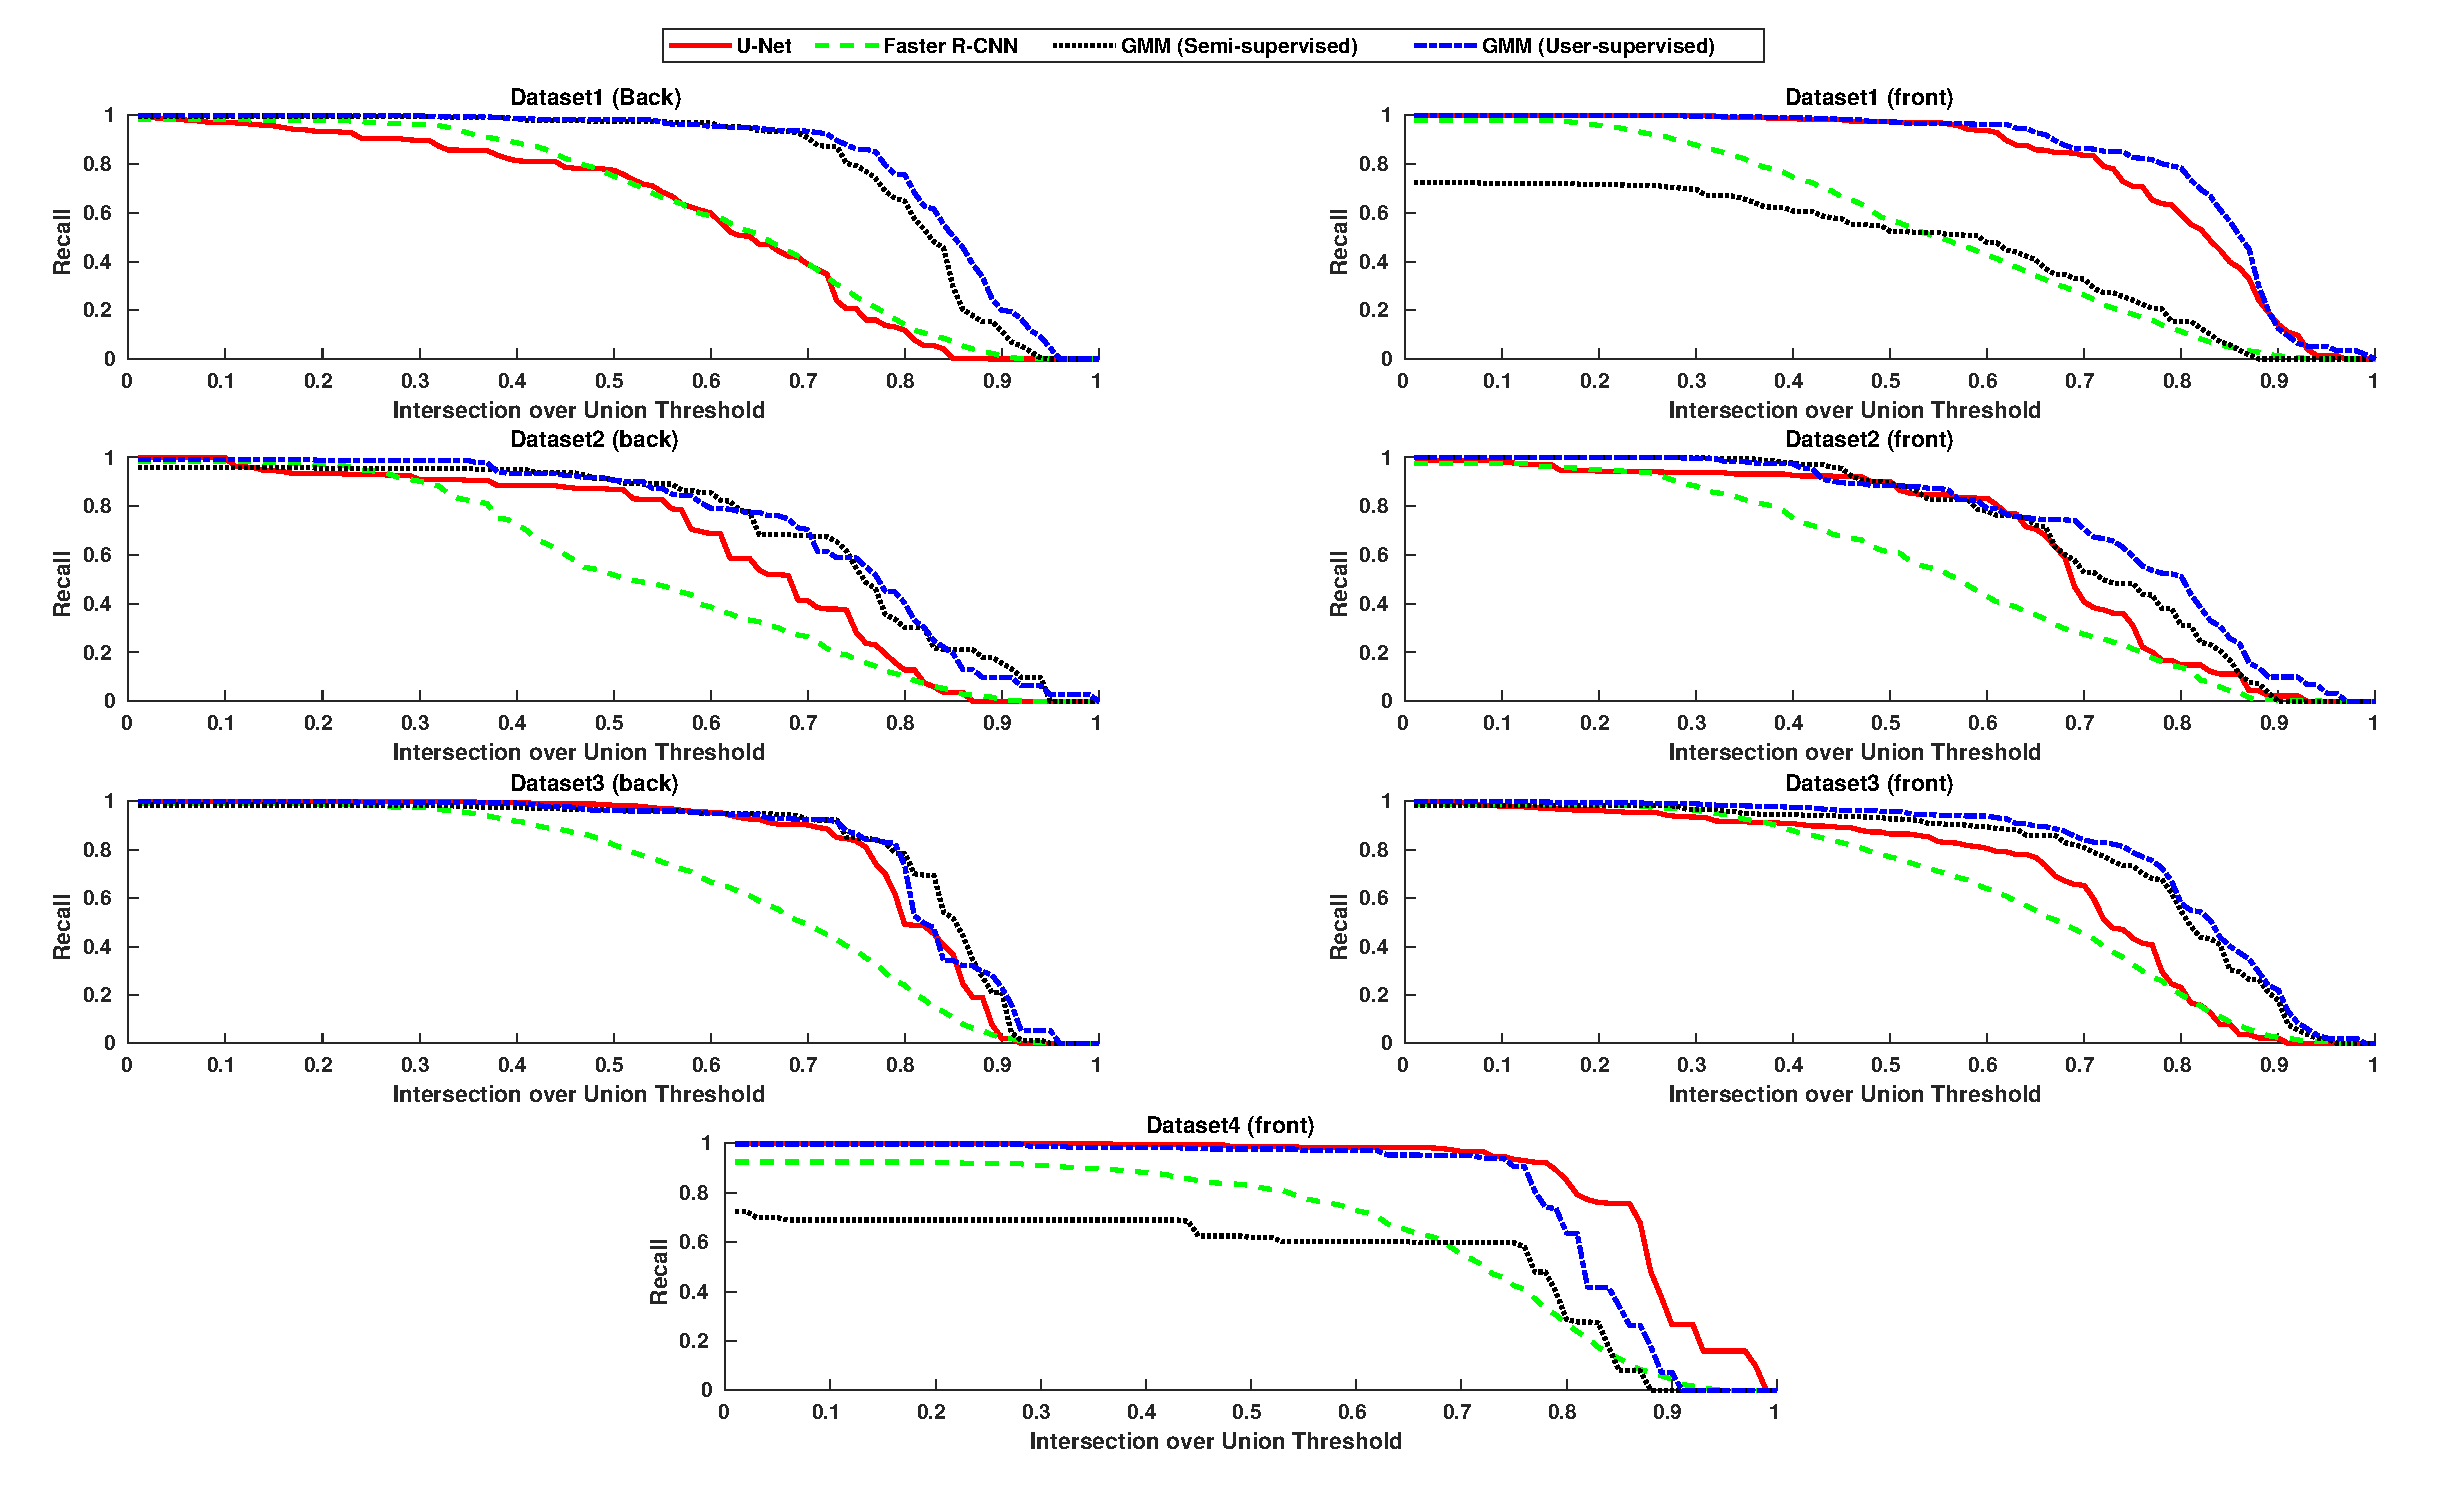
\includegraphics[width=\textwidth]{figures/detection/recall_with_semisup_gmm_.eps}
    \caption[Recall for the detection methods.]{Recall of the detection methods on all seven datasets}
    \label{fig:recall}
\end{figure}

The user-supervised GMM method outperforms the other three approaches on $6$ out of seven datasets and is competitive on the last one. This outcome is expected, as the training models were tuned for each test set. The reason it falls behind in Dataset4 (front) is since color features alone were not enough to detect all the fruits. The performance of the semi-supervised GMM depends on how closely the test set color space resembles the training model. In the case of Dataset1 (front) and Dataset4 (front) the color space of the test, set was different from the training model and therefore the recall drops substantially. In the other five test sets, the fruit colors and lighting conditions were similar to the training set and the model achieves similar recalls to the user-supervised model. 
Our proposed technique based on U-Net achieves consistently high recall for all the datasets. In Dataset4 (front) it even outperforms the user-supervised GMM. This success can be attributed to the use of non-color features. The FRCNN method also achieves high recall (especially in the low IoU region. This is consistent with \cite{bargoti_deep_2017}, who suggested to use the FRCNN with $IoU = 0.2$. 

When we look at the plots showing the precision in Fig.~\ref{fig:precision} the story is a different one. The user-supervised GMM approach outperforms the other three methods by a large margin in six out of seven test sets. The user-supervised GMM method is the only method to achieve precision values of $>90\%$ on all datasets. These high precisions can be attributed to the fact that the user supervisions were conservative and purposefully avoided ambiguous color clusters. The semi-supervised GMM achieves precision values of $>90\%$ in five out of seven datasets. For Dataset2 (back) and Dataset4 (front), the precision values fall under $80\%$ for all IoU levels. Again, this drop can be attributed to the dissimilarity in color space and lighting conditions between the train and test sets. 

\begin{figure}[!htbp]
    \centering
    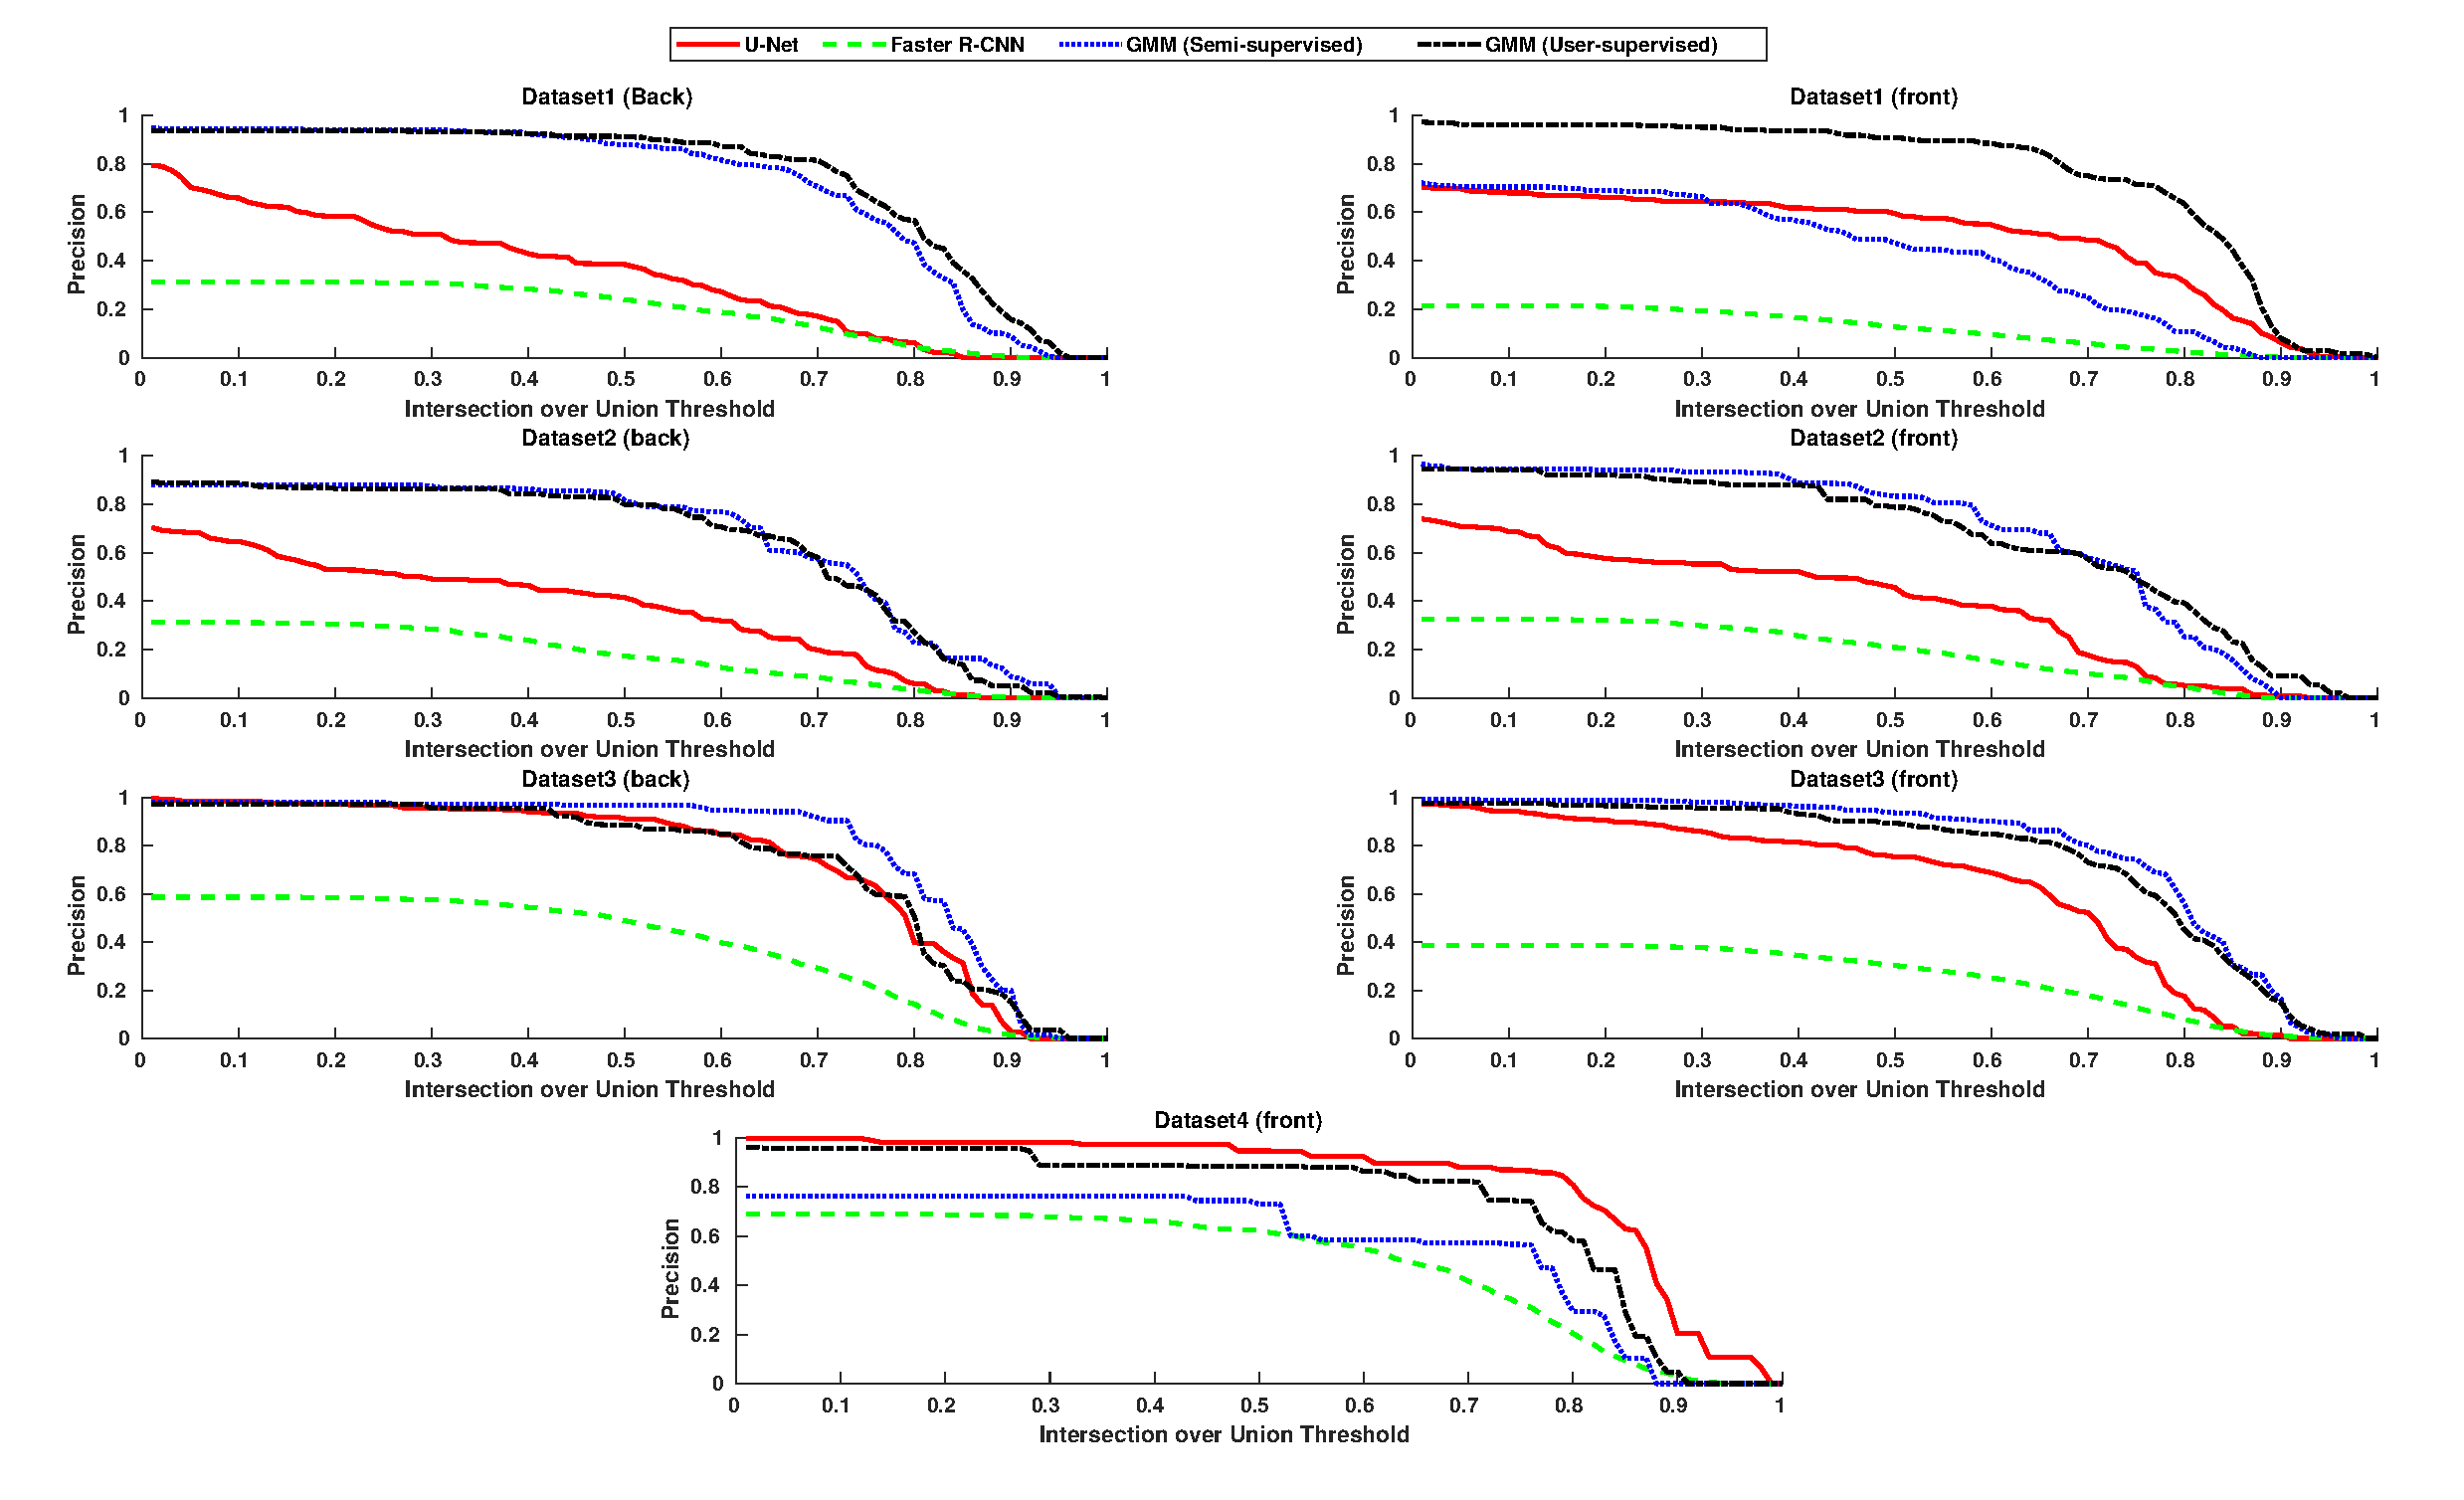
\includegraphics[width=\textwidth]{figures/detection/precision_with_semisup_gmm_.eps}
    \caption[Precision for the detection methods.]{Precision of the detection methods on all seven datasets}
    \label{fig:precision}
\end{figure}

The U-Net based approach does not achieve precision values over $80\%$ in four out of seven datasets. We show some examples of the false positives in Section~\ref{sec:qualitative}. From the qualitative results, we see that the network detects yellowing leaves as apples. The apple trees did not have any yellowing leaves during 2015, and consequently, our training data did not have any such examples. However, this problem can likely be solved by adding more training data. When color features alone were not enough to detect all the fruits, as in Dataset4 (front), the network has higher precision than all other methods. 
The FRCNN method has the lowest precision on all datasets even with low IoU. This is due to three reasons: First, the network detects more false positives than the other two methods. Second, the FRCNN often merges separate object instances into one. Third, the Non-Maximum Suppression (NMS) either filters out true positives or returns multiple detections for a single object instance. NMS is prone to such behavior due to the manual choice of its threshold. In Section~\ref{sec:qualitative} we show qualitative examples that illustrate this behavior.  
These findings again confirm \cite{bargoti_deep_2017}. In their work, they estimated that roughly $4\%$ of the total error could be attributed to the network's inability to distinguish between clustered fruits. Instead, they treat detections as clusters, not only as single fruits, which helps increase precision. Additionally, the FRCNN is the largest detection network and therefore suffers the most from the apparent shortage of training data.

Since $F_1$-measure combines recall and precision, we expect the user-supervised GMM to outperform the other three approaches on most of the datasets as seen in Fig.~\ref{fig:F1}. However, the U-Net detection approach achieves competitive $F_1$-measure on Dataset3 (back) and even outperforms the GMM approach on Dataset4 (front).

\begin{figure}[!htbp]
    \centering
    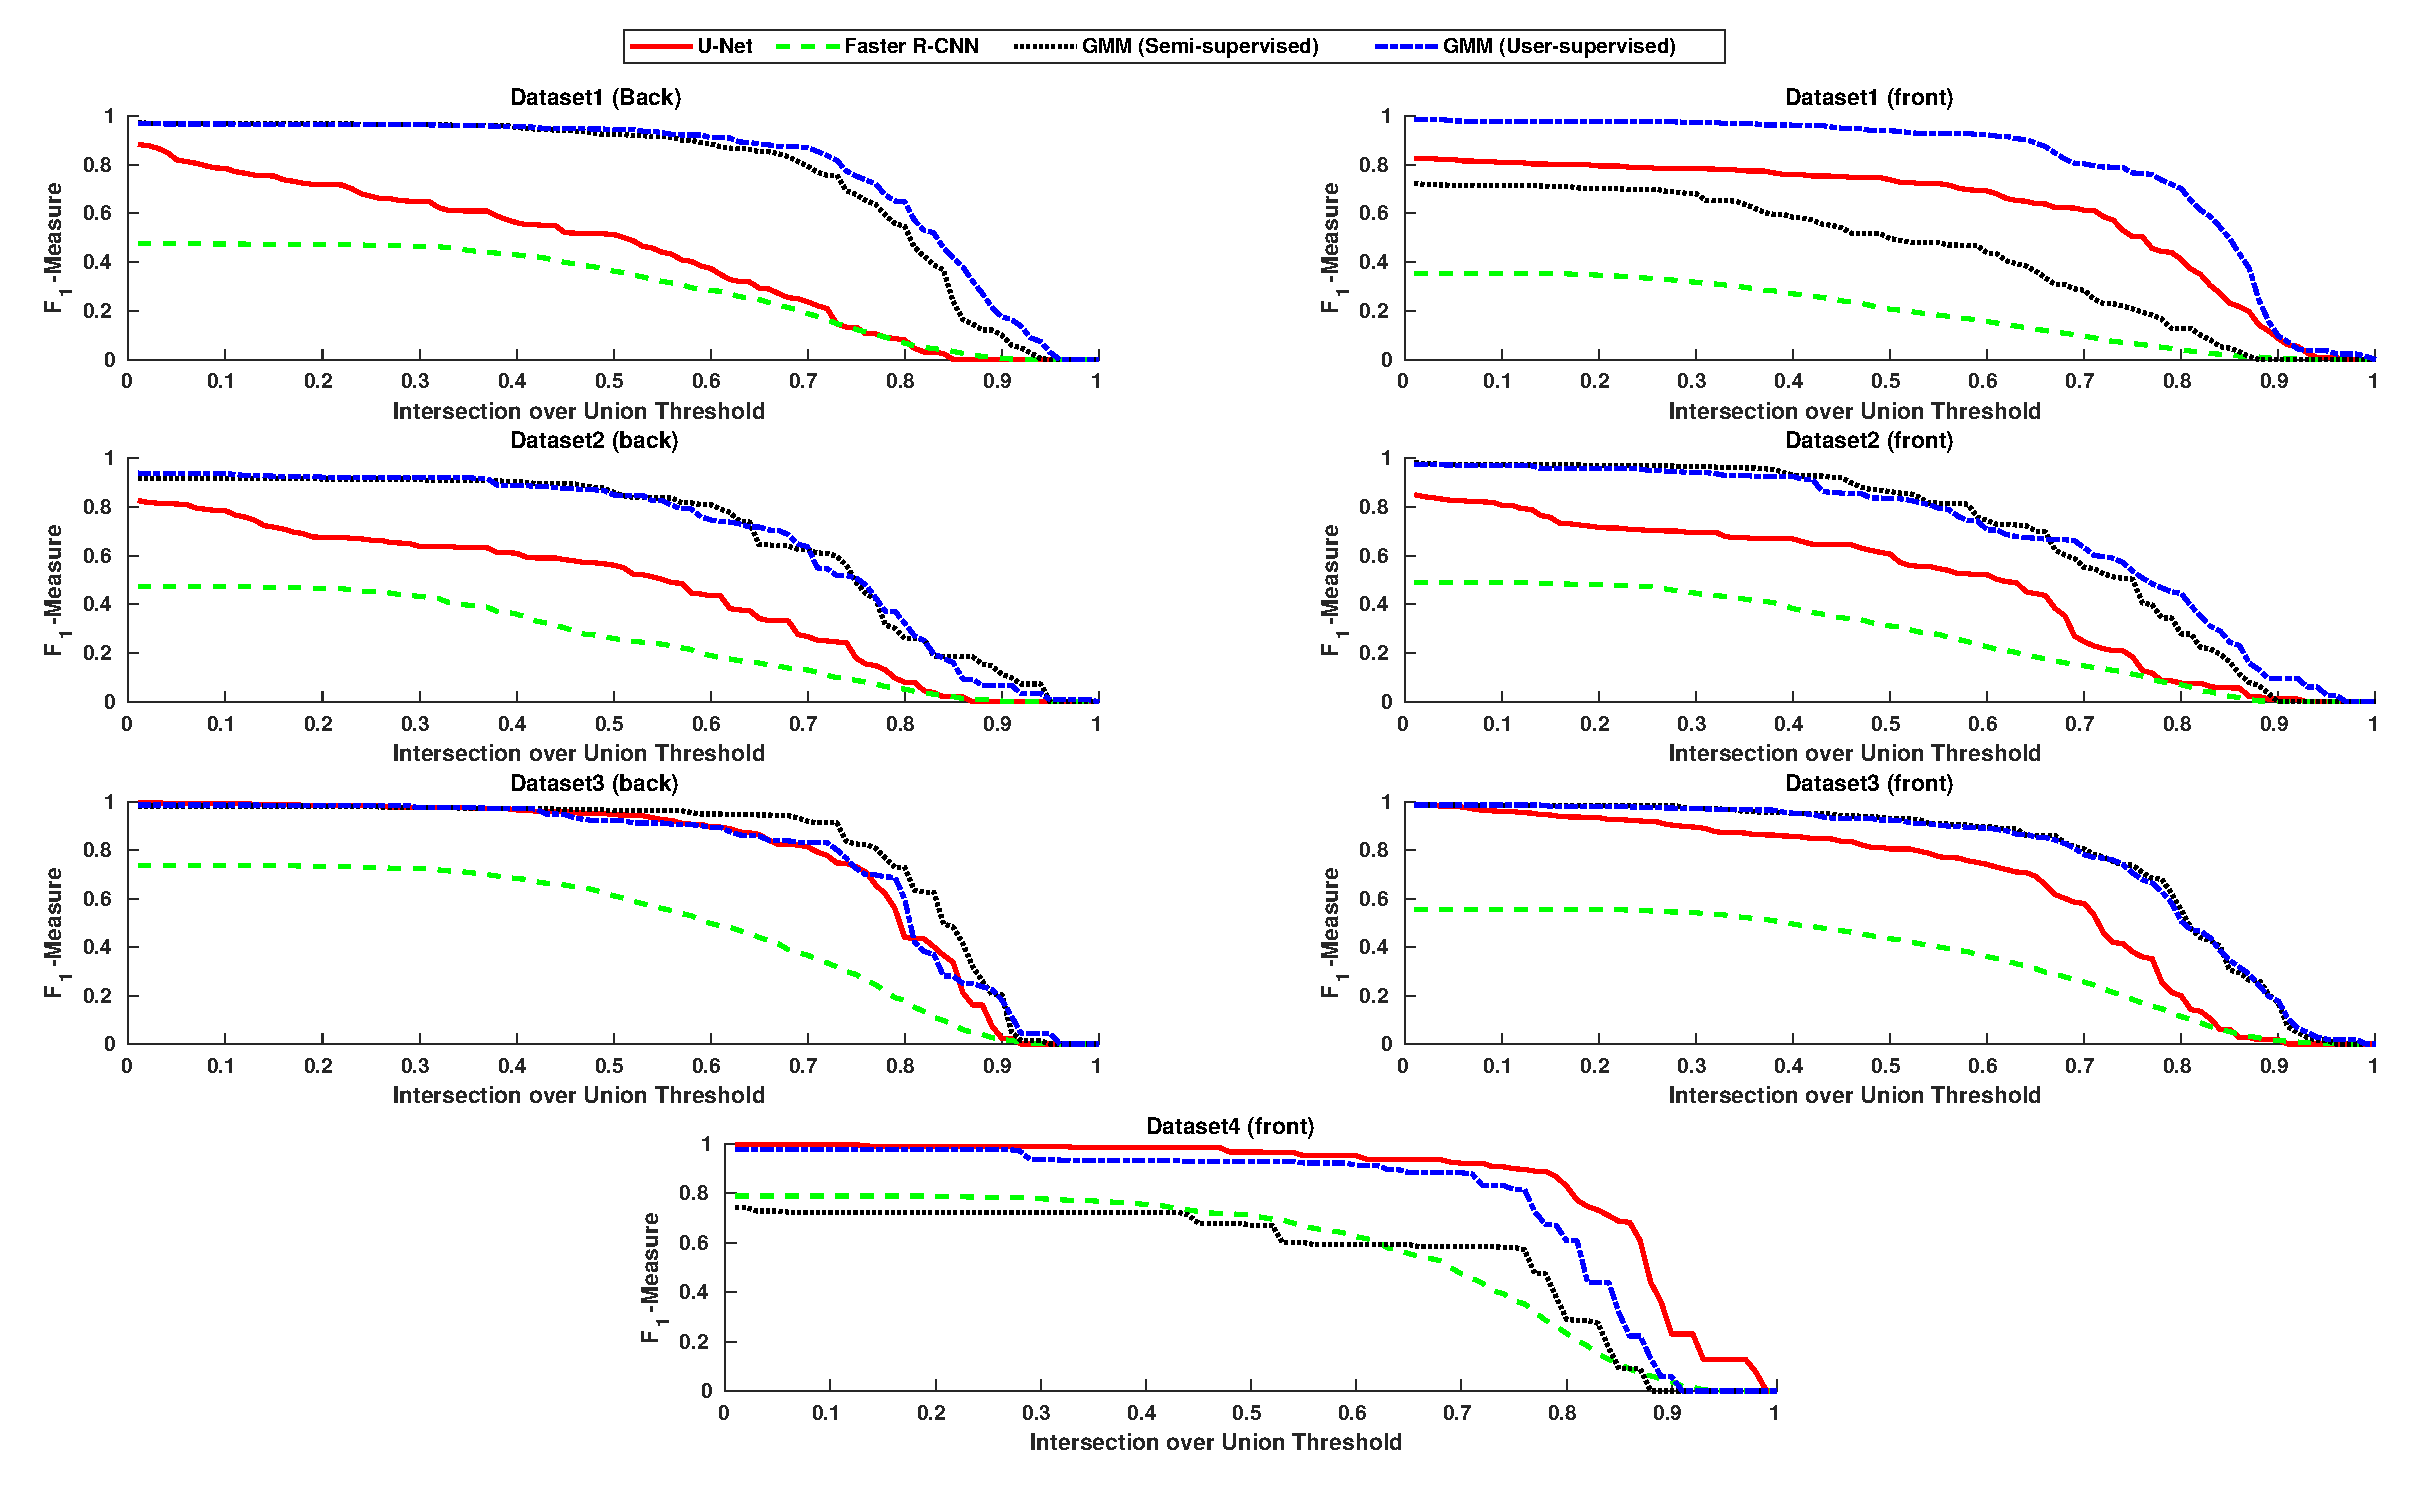
\includegraphics[width=\textwidth]{figures/detection/f1_with_semisup_gmm_.eps}
    \caption[$F_1$-measure for the detection methods.]{$F_1$-measure of the detection methods on all seven datasets}
    \label{fig:F1}
\end{figure}

After these extensive evaluations, we can conclude with conviction, that when fruits are distinguishable by colors, it is hard to beat the user-supervised GMM model. If color features are not good enough, we do need a more robust solution such as U-Net. However, the training set needs to cover a broader range of apple varieties, growth stages, and lighting conditions.

\subsubsection{Timing}
Detection performance is arguably the most important aspect of an object detection algorithm. A second aspect driving the choice of algorithm is its time complexity. The GMM approach runs at $5$ frames per second. The U-Net used in our experiments runs in less than 100 ms per image patch. We use image patches of size $224\times 224$ pixels with zero overlap. A full image of size $1920 \times 1080$ pixels takes less than $4.5$ seconds per frame.  For the FRCNN we follow the tiling approach proposed by~\cite{bargoti_deep_2017}. They use image crops of size $500 \times 500$ pixels with a stride of $50$ pixel. The FRCNN network takes $120$ ms per image patch. To detect objects in an image of $1920 \times 1080$ pixels takes up to $46$ seconds per frame. We acquire images at a rate of $30$ frames per second and move at a speed of $2$~m/s which renders the tiling approach infeasible for large orchards. These timings were measured on a conventional laptop with a single NVIDIA Quadro M1000 GPU.

\subsection{Qualitative Results}
\label{sec:qualitative}
In this section, we show some qualitative examples from three datasets. We illustrate the performance of the three detection approaches on a sample image from each of these datasets. In Dataset4 (front) color features alone were not enough to detect all the apples; causing problems for the user-supervised GMM. Dataset1 (front) contains many yellowing leaves causing problems for both the U-Net and FRCNN. On Dataset3 (back) both the GMM and U-Net achieved high precision and recall, but the FRCNN still had poor precision.

\begin{figure}[hbpt]
    \centering
    \def\svgwidth{0.82\textwidth}
    \import{figures/detection/}{qualitative.pdf_tex}
    \caption[Sample qualitative results for the detection methods.]{Some qualitative results for the proposed detection methods}
    \label{fig:qualitative}
\end{figure}

\subsection{Failure Cases}
In Section~\ref{sec:qualitative} we presented some qualitative examples. We now analyze the most common failure cases in more detail and offer insights into how these can be overcome in the future. Some common failure cases of the detection stage are shown in Fig.~{\ref{fig:failuregmm-unet}}.

\begin{figure}[htb]
    \centering
    \includegraphics[width=\textwidth]{figures/detection/failure_cases_detection.eps}
    \caption[Common failure cases of the detection methods.]{Common failure cases of the three evaluated detection methods}
    \label{fig:failuregmm-unet}
\end{figure}

The three methods have similar causes of errors, namely grouping of object instances, false-positive detections and false negatives. In addition to these cases, deep learning-based methods also split single objects into multiple detections. For the U-Net and the GMM detection methods, the additional network in the counting stage provides the means to reject false positives in $\sim 85\%$ of the cases. The FRCNN method does not contain an additional network for counting. However, the FRCNN could be changed to classifying instances into cluster counts instead of fruit/background. Such an approach will solve the problem of grouped instances and can reject false positives. However, doing so is not straightforward. Future research would have to determine how to merge overlapping predictions and set up an adequate training procedure.

The problem of false negatives is a more challenging one. It occurs in all three detection methods, but for different reasons. In the GMM-based detection method, the number of clusters to over-segment the images are chosen by the user a priori. If this threshold is too low, the model lacks the representative power to disambiguate among different object categories. If the threshold is too high, developing a training model becomes tedious, as many color clusters are required to capture all the fruits. In some cases, the fruits might not be distinguishable by color at all.
In the case of the U-Net and the FRCNN, this phenomenon is in part due to a lack of training data. The number of false positives for both of these methods highest on Dataset 1. Acquired in late September, the leaves in this dataset were turning yellow. The change of color impacts the networks' performance due to a lack of similar examples in the training set. An additional reason for false negatives in the FRCNN approach is the usage of Non-Maximum Suppression (NMS). Since NMS uses static thresholds, the network is prone to filter out overlapping true positives. While NMS is the de-facto standard algorithm to reject overlapping instances, it hurts performance when we try to detect individual instances of grouped objects.

\section{Experimental Insights and Conclusion}\label{sec:detection_conc}

In this chapter, we presented two different methods for fruit detection. The semi-supervised clustering technique, based on Gaussian Mixture Model (GMM) achieved the highest $F_1$-score in six out of seven datasets. The approach based on U-Net performed reasonably well, but Faster R-CNN suffered from poor precision. Our results provide quantitative insights into how much we gain in terms of performance with deep learning approaches. When fruits are distinguishable by color, the semi-supervised detection method outperformed both the U-Net and FRCNN. The U-Net approach performed exceedingly well when the test dataset was similar to the training dataset (for example U-Net on Dataset 4 (front)). However, for fruit detection, many challenges remain. It has hard to offer conclusive insights towards the generalizability of the U-Net and FRCNN approaches based on the limited amount of data we had available for training. We need to increase the size of the training data to gain more insights into this question.

Obtaining more data involves labeling fruit boundaries in images and labeling by skilled laborers is time-intensive and costly. To eliminate the painstaking process of labeling, we study realistic synthetic data generation in Chapter~\ref{chapter:semgan}. In the next chapter, we present a method for counting fruit in the detected clusters.